\documentclass[12pt]{article}
\usepackage{amsmath}
\usepackage{xcolor}
\usepackage{tikz}
\usepackage{geometry}
\geometry{margin=1in}

% Define NCERT blue color
\definecolor{ncertblue}{RGB}{0,112,192}

% Remove paragraph indentation
\setlength{\parindent}{0pt}

\begin{document}
\begin{figure}[h!]
    \begin{minipage}{0.45\textwidth}  % Set the width of the image
        \includegraphics[width=\textwidth]{ki.png}  % Replace 'image.png' with your image file name
    \end{minipage} \hfill
    \begin{minipage}{0.45\textwidth}  % Set the width of the text block
        \textbf{Name : K.VINOD KUMAR REDDY} \\
    \textbf{Batch : cometfwc0025} \\
  \textbf{Date : 15th MAY 2025}
    \end{minipage}
\end{figure}
% Example 1
\noindent\textcolor{ncertblue}{\textbf{Example 1:}} Do the points \( (3, 2) \), \( (-2, -3) \) and \( (2, 3) \) form a triangle? If so, name the type of triangle formed.

\vspace{1em}

\noindent\textcolor{ncertblue}{\textbf{Solution:}} Let us apply the distance formula to find the distances \( PQ \), \( QR \), and \( PR \), where \( P(3, 2) \), \( Q(-2, -3) \) and \( R(2, 3) \) are the given points. We have

\[
PQ = \sqrt{(3+2)^2 + (2+3)^2} = \sqrt{5^2 + 5^2} = \sqrt{50} = 7.07 \text{ (approx.)}
\]

\[
QR = \sqrt{(-2 - 2)^2 + (-3 - 3)^2} = \sqrt{(-4)^2 + (-6)^2} = \sqrt{52} = 7.21 \text{ (approx.)}
\]

\[
PR = \sqrt{(3 - 2)^2 + (2 - 3)^2} = \sqrt{1^2 + (-1)^2} = \sqrt{2} = 1.41 \text{ (approx.)}
\]

Since the sum of any two of these distances is greater than the third distance, the points \( P \), \( Q \), and \( R \) form a triangle.\\
Also, \( PQ^2 + PR^2 = QR^2 \). By the converse of Pythagoras' theorem, we have \( \angle P = 90^\circ \).\\
Therefore, \( \triangle PQR \) is a right triangle.

\vspace{3em}

% Example 3 statement
\noindent\textcolor{ncertblue}{\textbf{Example 3 :}} Fig. 7.6 shows the arrangement of desks in a classroom. Ashima, Bharti and Camella are seated at \( A(3, 1) \), \( B(6, 4) \), and \( C(8, 6) \) respectively. Do you think they are seated in a line? Give reasons for your answer.

\vspace{1em}

% Fig 7.6: grid with points
\begin{center}
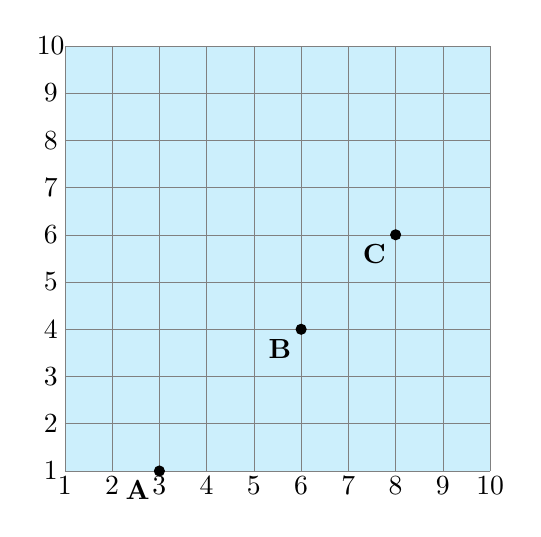
\begin{tikzpicture}[scale=0.6]
  % Light blue background for grid
  \fill[cyan!20] (1,1) rectangle (10,10);

  % Draw grid lines
  \draw[step=1cm,gray,very thin] (1,1) grid (10,10);

  % Points A, B, C with labels
  \filldraw[black] (3,1) circle (3pt) node[below left] {\textbf{A}};
  \filldraw[black] (6,4) circle (3pt) node[below left] {\textbf{B}};
  \filldraw[black] (8,6) circle (3pt) node[below left] {\textbf{C}};

  % Numbering for columns and rows
  \foreach \x in {1,...,10} {
    \node at (\x,0.7) {\x};
  }
  \foreach \y in {1,...,10} {
    \node at (0.7,\y) {\y};
  }
\end{tikzpicture}

\vspace{0.3em}
\textcolor{ncertblue}{\textbf{Fig. 7.6}}
\end{center}

\vspace{1em}

% Solution part
\noindent\textcolor{ncertblue}{\textbf{Solution :}} Using the distance formula, we have
\[
\begin{aligned}
AB &= \sqrt{(6 - 3)^2 + (4 - 1)^2} = \sqrt{9 + 9} = \sqrt{18} = 3\sqrt{2} \\
BC &= \sqrt{(8 - 6)^2 + (6 - 4)^2} = \sqrt{4 + 4} = \sqrt{8} = 2\sqrt{2} \\
AC &= \sqrt{(8 - 3)^2 + (6 - 1)^2} = \sqrt{25 + 25} = \sqrt{50} = 5\sqrt{2}
\end{aligned}
\]

Since \( AB + BC = 3\sqrt{2} + 2\sqrt{2} = 5\sqrt{2} = AC \), we can say that the points A, B and C are collinear. Therefore, they are seated in a line.

\end{document}
